\documentclass{amsart}
\usepackage[utf8]{inputenc}
\usepackage[english]{babel}
\usepackage{amsmath}
\usepackage{tikz-cd}

\newtheorem{theorem}{Theorem}
\newtheorem{lemma}[theorem]{Lemma}
\theoremstyle{definition}
\newtheorem{definition}[theorem]{Definition}

\newcommand{\N}{\mathbb{N}}
\newcommand{\Z}{\mathbb{Z}}
\newcommand{\R}{\mathbb{R}}
\newcommand{\HS}{\mathrm{HS}}
\newcommand{\dprime}{{\prime\prime}}
\DeclareMathOperator{\im}{im}
\DeclareMathOperator{\interior}{int}

\setlength{\textwidth}{\paperwidth}
\addtolength{\textwidth}{-1.4in}
\setlength{\textheight}{\paperheight}
\addtolength{\textheight}{-1.8in}
\calclayout

\newcommand{\p}{\mathrm{p}}
\newcommand{\q}{\mathrm{q}}

\usepackage{parskip}
\begin{document}

\begin{definition}
	For $n \in \N$, a continuous map is said to be \textit{$n$-homologically small}, denoted $\HS_n$, if the image of the map induced by $H_n(-)$ is finitely generated, and we say it is \textit{homologically small}, denoted $\HS$, if it is $\HS_n$ for every $n$.
\end{definition}

\begin{definition}
	Let $X$ be a space and $f \colon X \to \R$ a function. For any $t \in \R$, the \textit{$t$-sublevel set of $f$} is defined by 
	\begin{equation*}
	X_{\leq t} = f^{-1}((-\infty, t]).
	\end{equation*}
\end{definition}

\begin{definition}
	Let $M$ be a metric space. For any $p \in M$ and $\epsilon > 0$, the \textit{$\epsilon$-neighborhood of $p$} is defined by
	\begin{equation*}
	B_\epsilon(p) = \{q \in M\ |\ d(p,q) < \epsilon\}.
	\end{equation*}
\end{definition}

\begin{definition}
	Let $M$ be a metric space and $f \colon M \to \R$ a function.
	The space $M$ is said to be \textit{strongly locally-$f$-connected} if for each $p \in M$, $e > 0$, and $n \in \N$ there exists $\delta \in (0, e)$ such that for every $c \geq 0$ the image of the map induced by $H_n(-)$ on $B_\delta(p) \cap M_{\leq f(p)+\delta+c} \to B_e(p) \cap M_{\leq f(p)+e+c}$ is $0$.
\end{definition}

\begin{theorem} \label{t:strong local connectenss implies tameness}
	Let $M$ be a metric space and $f \colon M \to \R$ a function. If $M$ is strongly locally-$f$-connected and all level sets are compact, then, for any $s < t$ the inclusion $M_s \to M_t$ is $\HS$.
\end{theorem}

\begin{lemma} \label{l:commutative algebra}
	Lemma 17.3 in Bredon.	
\end{lemma}

\begin{lemma}
	Let $M$ and $f$ be as in Theorem \ref{t:strong local connectenss implies tameness}.
	For compact sets $K, L \subseteq M$ with $K \subseteq \interior(L)$ and $s < t$ there is $\delta \in (0,\, t-s)$ such that $K \cap M_{s+\delta} \to L \cap M_{t}$ is $\HS$.
\end{lemma}

\begin{proof}
	We will proceed by induction on $n \in \N$. Assume the lemma holds with $\HS$ replaced with $\HS_{(n-1)}$.
	Given a compact set $L \subseteq M$ and $s < t$ let $\Sigma_{s, t}$ be the collection of all compact subsets $K$ of $M$ for which there exists $\delta_K > 0$ and an open neighborhood $U_K$ of $K$ such that $U_K \cap M_{s+\delta_K} \to L \cap M_{t}$ is $\HS_n$.
	
	We start by showing that any point in $\interior(L) \cap M_s$ has a neighborhood in $\Sigma_{s, t}$.
	Let $x \in \interior(L) \cap M_{s}$ and take $e > 0$ such that $s + e < t$ and $B_e(x) \subseteq \interior(L)$.
	By the strong local-$f$-connectivity of $M$, there exists $\delta \in (0, e)$ such that for $c = s - f(x)$ and any $d \geq 0$ the following composition is $\HS$:
	\begin{equation*}
	B_\delta(x) \cap M_{s + \delta + d} =
	B_\delta(x) \cap M_{f(x) + c + \delta + d} \to
	B_e(x) \cap M_{f(x) + c + e + d} \to
	L \cap M_{t + d}.
	\end{equation*}  
	
	We will now show that the class $\Sigma_{s,t}$ is closed under finite unions.
	For $i = 1, 2$ let $K_i \in \Sigma_{s,t}$ with chosen $\delta_i > 0$ and open neighborhood $U_i$. Let $K_i^\dprime$ and $K_i^\prime$ be compact sets such that
	\begin{equation*}
	K_i \subseteq \interior(K_i^\dprime) \subseteq K_i^\prime \subseteq U_i,
	\end{equation*}
	which can be easily constructed using that any neighborhood of a point in a metric space contains a compact neighborhood of that point.
	Notice that, since $K_i \subseteq U_i$, if $\delta = \min(\delta_i)$ then $K_i^\prime \cap M_{s+\delta} \to L \cap M_t$ is $\HS_n$ and that by induction we have that $K_1^\dprime \cap K_2^\dprime \cap M_s \to K_1^\prime \cap K_2^\prime \cap M_{s+\delta}$ is $\HS_{(n-1)}$.
	
	We therefore have the following commutative diagram satisfying the assumptions of Lemma \ref{l:commutative algebra}:
	\begin{equation*}
	\begin{tikzcd}
	& H_n(L \cap M_t) & \arrow[l] H_n(L \cap M_t) \oplus H_n(L \cap M_t) \\
	H_{n-1}(K_1^\prime \cap K_2^\prime \cap M_{s+\delta}) & 
	H_{n}((K_1^\prime \cap M_{s+\delta}) \cup (K_2^\prime \cap M_{s+\delta})) \arrow[l] \arrow[u] &
	H_{n}(K_1^\prime \cap M_{s+\delta}) \oplus H_n(K_2^\prime \cap M_{s+\delta}) \arrow[l] \arrow[u] \\
	H_{n-1}(K_1^\dprime \cap K_2^\dprime \cap M_s) \arrow[u] & 
	H_{n}((K_1^\dprime \cap M_s) \cup (K_2^\dprime \cap M_s)), \arrow[l] \arrow[u] &
	\end{tikzcd}
	\end{equation*}
	which implies $K_1 \cup K_2 \in \Sigma_{s, t}$ as desired. Since any $K \subseteq \interior(L)$ can be expressed as a finite union of sets in $\Sigma_{s,t}$ the lemma is proven.
\end{proof}

\newpage

Assume $X$ is Hausdorff and locally compact.

Let $p_n$ be the proposition: For compact sets $K, L \subseteq X$ with $K \subseteq \interior(L)$, $\forall s < t$, $\exists\, \delta \in (0, t-s)$ s.t. $K \cap M_{s+\delta+c} \to L \cap M_{t+c}$ is $n$-fgi for $c \geq 0$.

Assume $(\ast): \forall x \in X$, $\forall e > 0$, $\exists \delta \in (0,e)$ s.t. $\forall c \geq 0$
\begin{equation*}
B_\delta(x) \cap M_{f(x)+\delta+c} \to B_e(x) \cap M_{f(x)+e+c}
\end{equation*} 
is $n$-fgi for all $n \geq 0$.

Given compact $L \subseteq X$, for $s < t$ let
\begin{equation*}
\Sigma_{s,t} = \{K \text{ compact}\ |\ \exists\, \delta \in (0, t-s), \exists\, K \subseteq U \subseteq \interior(L) \text{ open s.t. } U \cap M_{s+\delta+c} \to L \cap M_{t+c} \text{ is $n$-fgi for } c\geq 0\}.
\end{equation*}

1) If $\interior(L) \cap M_s \neq \emptyset$ then $\Sigma_{s, t}$ is not empty:

Let $x \in \interior(L) \cap M_{s}$ and take $e > 0$ such that $s + e < t$ and $B_e(x) \subseteq \interior(L)$.
By $(\ast)$ there exists $\delta \in (0, e)$ such that for $c = s - f(x)$ and any $d \geq 0$ the following composition is $n$-fgi for any $n$
\begin{equation*}
B_\delta(x) \cap M_{s + \delta + d} =
B_\delta(x) \cap M_{f(x) + c + \delta + d} \to
B_e(x) \cap M_{f(x) + c + e + d} \to
L \cap M_{t + d}.
\end{equation*}  

2) $\Sigma_{s,t}$ is closed under finite unions:

For $i = 1, 2$, let $K_i \in \Sigma_{s,t}$ with associated $\delta_i$ and $U_i$. Let $K_i^\dprime$ and $K_i^\prime$ be compact sets such that
\begin{equation*}
K_i \subseteq \interior(K_i^\dprime) \subseteq K_i^\prime \subseteq U_i.
\end{equation*}
Notice that if $\delta = \min(\delta_i)$ then $K_i^\prime \cap M_{s+\delta} \to L \cap M_t$ is $n$-fgi.

\begin{equation*}
\begin{tikzcd}
& H_n(L \cap M_t) & \arrow[l] H_n(L \cap M_t) \oplus H_n(L \cap M_t) \\
H_{n-1}(K_1^\prime \cap K_2^\prime \cap M_{s+\delta}) & 
H_{n}((K_1^\prime \cap M_{s+\delta}) \cup (K_2^\prime \cap M_{s+\delta})) \arrow[l] \arrow[u] &
H_{n}(K_1^\prime \cap M_{s+\delta}) \oplus H_n(K_2^\prime \cap M_{s+\delta}) \arrow[l] \arrow[u] \\
H_{n-1}(K_1^\dprime \cap K_2^\dprime \cap M_s) \arrow[u] & 
H_{n}((K_1^\dprime \cap M_s) \cup (K_2^\dprime \cap M_s)) \arrow[l] \arrow[u]. &
\end{tikzcd}
\end{equation*}

\newpage

Assume $X$ is Hausdorff and locally compact.

Let $p_n$ be the proposition: For compact sets $K, L \subseteq X$ with $K \subseteq \interior(L)$, $\forall s < t$, $K \cap Y_{s+c} \to L \cap Y_{t+c}$ is $n$-fgi for $c \geq 0$.

Assume $(\ast): \forall x \in X$, $\forall e > 0$, $\exists \delta \in (0,e)$ s.t. $\forall c \geq 0$
\begin{equation*}
B_\delta(x) \cap Y_{f(x)+\delta+c} \to B_e(x) \cap Y_{f(x)+e+c}
\end{equation*} 
is $n$-fgi for all $n \geq 0$.

Given compact $L \subseteq X$, for $s < t$ let
\begin{equation*}
\Sigma_{s,t} = \{K \text{ compact}\ |\ \exists\ K \subseteq U \subseteq \interior(L) \text{ open s.t. } U \cap Y_{s+c} \to L \cap Y_{t+c} \text{ is $n$-fgi for } c\geq 0\}.
\end{equation*}

1) If $\interior(L) \cap Y_s \neq \emptyset$ then $\Sigma_{s, t}$ is not empty:

Let $x \in \interior(L) \cap Y_{s}$ and take $e > 0$ such that $s + e < t$ and $B_e(x) \subseteq \interior(L)$.
By $(\ast)$ there exists $\delta \in (0, e)$ such that for $c = s - f(x)$ and any $d \geq 0$ the following composition is $n$-fgi for any $n$
\begin{equation*}
B_\delta(x) \cap Y_{s + d} \to
B_\delta(x) \cap Y_{f(x) + c + \delta + d} \to
B_e(x) \cap Y_{f(x) + c + e + d} \to
L \cap Y_{t + d}.
\end{equation*}  

2) $\Sigma_{s,t}$ is closed under finite unions:

Let $K_1, K_2 \in \Sigma_{s,t}$ we will construct for $i=1, 2$ compact sets $K_i^\prime$ such that
\begin{equation*}
K_i \subseteq \interior(K_i^\prime) \subseteq K_i^\prime
\end{equation*}
and $K_i^\prime \cap Y_{s+\epsilon} \to L \cap Y_t$ is $n$-fgi.

Issue about the fact that $U_i \cap Y_{s+\epsilon} \to L \cap Y_{t+\epsilon}$ is $n$-fgi but not $s+\epsilon \to t$ as needed for the induction.

\newpage

%	Let $f$ be a real-valued function from a metric space $M$ such that for every $s \in \R$ the preimage $M_{\leq s} = f^{-1}(\{r \leq s\})$ is compact and satisfies the following property:\\
%	
%	Given values $s < t$, a point $p \in M_{\leq s}$, and any open neighborhood $V$ of $p$ in $M_{\leq t}$ there is an open neighborhood $U \subseteq V$ of $p$ such that $\im \big(\widetilde H_\bullet(U \cap M_{\leq s}) \to \widetilde H_\bullet(V)\big) = 0$.\\
%	
%	Then, $\im \big(H_d(Y) \to H_d(X)\big)$ is finitely generated for every $d$.\\
%	
%	Take $s < t$. If there exists $t_i \in (s, t]$ such that $M_{\leq s} = M_{\leq t_1}$ we are done by Wilder's original theorem.
%	
%	Assume the contrary. 
	
	We use the following terminology: a \textit{neighborhood} of a point is a set containing an open neighborhood of it.
	
	\begin{lemma} 
		Let $Y_t$ a filtration by compact subsets of a locally compact and Hausdorff space $X$. Define the following properties:
		\begin{itemize}
			\item[$\p(n)$] Let $s < t$. If $K$ and $L$ are compact subsets of $X$ with $K \cap Y_s \subset \interior(L) \cap Y_t$, then $\im H_n\left(K \cap Y_s \to L \cap Y_t\right)$ is finite.
			\item[$\q(n)$] Let $s < t$. If $V$ is an open neighborhood of $y \in Y_s$, then there exist an open set $U \subseteq V$ such that $\im H_n\left(U \cap Y_s \to V \cap Y_t\right)$ is finite.
		\end{itemize}
		Then, $\p(n-1)$ together with $\q(n)$ imply $\p(n)$.
	\end{lemma}
	
	\begin{proof}
		Recall the following fact:
		$(\ast)$ A space $S$ if locally compact and Hausdorff if and only if for every point $p$ of $S$, any neighborhood of $p$ contains a compact neighborhood of $p$.
		
		Let $K$ and $L$ as above and choose $r \in (s, t)$. Using $\q(n)$ for $r < t$ we can choose for each $y \in Y_r$ an open $U(y)$ such that $U(q) \cap Y_r \to \interior(L) \cap Y_t$ is $H_n$-finite. Let $D(y) \subseteq U(y)$ be a compact neighborhood of $y$. Using $\q(n)$ for $s < r$ consider for any $x \in Y_s \subseteq Y_r$ an open neighborhood $W(x) \subseteq \interior(D(x))$ such that $W(x) \cap Y_s \to \interior(D(x)) \cap Y_t$ is $H_n$-finite. Denote by $C(x) \subseteq W(x)$ a compact neighborhood of $x$. Notice that for any $x, x^\prime \in Y_s$ we have $C(x) \cap C(x^\prime) \cap Y_s \subseteq \interior(D(x) \cap D(x^\prime)) \cap Y_r$. So, by $\p(n-1)$, the inclusion map $C(x) \cap C(x^\prime) \cap Y_s \to \interior(D(x) \cap D(x^\prime)) \cap Y_r$ is $H_{n-1}$-finite.
		\begin{equation*}
		\begin{tikzcd}
		& H_n(L \cap Y_r) & \arrow[l] H_n(L \cap Y_r) \oplus H_n(L \cap Y_r) \\
		H_{n-1}(D_1 \cap D_2 \cap Y_t) & 
		H_n((D_1 \cap Y_t) \cup (D_2 \cap Y_t)) \arrow[l] \arrow[u] &
		\arrow[l] H_n(D_1 \cap Y_t) \oplus H_n(D_2 \cap Y_t) \arrow[u] \\
		H_{n-1}(C_1 \cap C_2 \cap Y_s) \arrow[u] & 
		H_n((C_1 \cap Y_s) \cup (C_2 \cap Y_s)) \arrow[l] \arrow[u]. &
		\end{tikzcd}
		\end{equation*}
		
		The upper right square has finite image because $\im H_n\left(K^\prime_i \cap Y \to M\right)$ is finite for each $i \in \{1, 2\}$. The bottom left square has a finite image using property $(r^{n-1})$. From standard homological algebra (cite Bredon 	Lemma 17.3) using that the middle row is exact, part of the Mayer-Vietoris sequence for the space $(K_1^\prime \cap Y) \cup (K_2^\prime \cap Y) \subseteq Y$, we conclude that $K = K_1 \cup K_2 \in \sigma$ with open neighborhood $U_K = \interior K^\dprime_1 \cup \interior K^\dprime_2$.
		
		Let $K$ be a compact set such that $\widetilde K = K \cap Y \subset \interior_Y(M \cap Y)$.
		Consider a finite subset $\{C_1, \dots, C_m\}$ of $\sigma$ such that $Y = \bigcup_{i=1}^m C_i \cap Y$. This set can be constructed using that $Y$ is compact and that any $y \in Y$ has a neighborhood in $\sigma$. Denoting $C = \bigcup_{i=1}^m C_i$ and $D = X \setminus \interior(C)$ we have $K = (K \cap C) \cup (K \cap D)$ which imply $K \in \sigma$ since $D \cap Y = \emptyset$ so $K \cap D \in \sigma$ trivially.
	\end{proof}


	
	
	
	
	
	
	
	
	
	
	
	
	
	
	
	
	
	
	
	
	
	
	
	
	
	\newpage
	
	We use the following terminology: a \textit{neighborhood} of a point is a set containing an open neighborhood of it.
	
	\begin{lemma} \label{l: wilder}
		Let $X$ be locally compact and Hausdorff and $Y \subseteq X$ compact. Define the following properties:
		\begin{itemize}
			\item[$(r^n)$] If $K$ and $M$ are compact subsets of $X$ with $K \cap Y \subset \interior_Y(M \cap Y)$, then $\im H_n\left(K \cap Y \to M\right)$ is finite.
			\item[$(r^n_\bullet)$] If $V$ is an open neighborhood of $y \in Y$, then there exist $U$ an open neighborhood of $y$ contained in $V$ such that $\im H_n\left(U \cap Y \to V\right)$ is finite.
		\end{itemize}
		Then, $(r^{n-1})$ together with $(r^n_\bullet)$ imply $(r^n)$.
	\end{lemma}
	
	\begin{proof}
		Let $M$ be fixed and let $\sigma$ be the set of compact subsets $K$ with $K \cap Y \subseteq \interior_Y(M \cap Y)$ such that $K$ has a neighborhood $U_K$ in $X$ such that $\im H_n\left(U_K \cap Y \to M\right)$ is finite.
		
		Recall the following fact:
		$(\ast)$ A space $S$ if locally compact and Hausdorff if and only if for every point $p$ of $S$, any neighborhood of $p$ contains a compact neighborhood of $p$.
		
		The collection $\sigma$ is not empty, in fact, it contains a compact neighborhood of any $y \in Y$. This follows from taking $V = X$ in $(r_\bullet^n)$ and using $(\ast)$ on the resulting open neighborhood.
		
		Notice that the collection $\sigma$ is closed under intersections. In fact, a stronger statement holds: if $K_1$ is compact and $K_2 \in \sigma$ then $K_1 \cap K_2 \in \sigma$. This is a consequence of the fact that the image of a map is finite can be deduced from that property holding for any map that factors it. We will next show that $\sigma$ is also closed under finite unions.
		
		For $i \in \{1, 2\}$ consider $K_i \in \sigma$ and let $K_i^\prime$ and $K_i^\dprime$ be compact neighborhoods of $K_i$ such that
		\begin{equation*}
		K_i \subseteq K_i^\dprime \subseteq \interior K_i^\prime \subseteq K_i^\prime \subseteq U_i,
		\end{equation*}
		where $\im H_n\left(U_i \cap Y \to M\right)$ is finite. 
		We can construct such compact neighborhoods using $(\ast)$ as follows:
		
		Consider for each $p \in K_i$ a compact neighborhood $K^\prime_i(p) \subseteq U_i$ and let $K_i^\dprime(p) \subseteq \interior K_i^\prime(p)$ be another compact neighborhood of $p$. The collection of open sets $\interior K_i^\dprime(p)$ covers the compact $K_i$. Let $\{p_i^{1}, \dots, p^{n}_i\} \subseteq K_i$ be such that $K_i \subseteq \bigcup_{j=1}^n \interior K^\dprime_i(p^j_i)$. Define $K_i^\dag = \bigcup_{j=1}^n K^\dag_i(p^j_i)$ for $i \in \{1,2\}$ and $\dag \in \{\prime, \dprime\}$.
		
		Furthermore, we have $K^\dprime_1 \cap K^\dprime_2 \cap Y \subseteq \interior_Y(K_1^\prime \cap K_2^\prime \cap Y)$. To see this consider $p \in K^\dprime_1 \cap K^\dprime_2 \cap Y$. By construction for $i \in \{1, 2\}$ there exist open sets $V_i \subseteq K_i^\prime$ such that $p \in V_i$. Letting $V = V_1 \cap V_2$ we have $p \in V \cap Y \subseteq K^\dprime_1 \cap K^\dprime_2 \cap Y$ implying $p \in \interior_Y(K^\dprime_1 \cap K^\dprime_2 \cap Y)$.
		
		\begin{equation*}
		\begin{tikzcd}
		& H_n(M) & \arrow[l] H_n(M) \oplus H_n(M) \\
		H_{n-1}(K_1^\prime \cap K_2^\prime) & 
		H_{n}(K_1^\prime \cup K_2^\prime) \arrow[l] \arrow[u] &
		H_{n}(K_1^\prime) \oplus H_n(K_2^\prime) \arrow[l] \arrow[u] \\
		H_{n-1}(K_1^\prime \cap K_2^\prime \cap Y) \arrow[u] & 
		H_{n}((K_1^\prime \cap Y) \cup (K_2^\prime \cap Y)) \arrow[l] \arrow[u] &
		H_{n}(K_1^\prime \cap Y) \oplus H_n(K_2^\prime \cap Y) \arrow[l] \arrow[u] \\
		H_{n-1}(K_1^\dprime \cap K_2^\dprime \cap Y) \arrow[u] & 
		H_{n}((K_1^\dprime \cap Y) \cup (K_2^\dprime \cap Y)) \arrow[l] \arrow[u]. &
		\end{tikzcd}
		\end{equation*}
		
%		\begin{equation*}
%		\begin{tikzcd}
%		& H_n(M) & \arrow[l] H_n(M) \oplus H_n(M) \\
%		H_{n-1}(K_1^\prime \cap K_2^\prime \cap Y) & 
%		H_{n}((K_1^\prime \cap Y) \cup (K_2^\prime \cap Y)) \arrow[l] \arrow[u] &
%		H_{n}(K_1^\prime \cap Y) \oplus H_n(K_2^\prime \cap Y) \arrow[l] \arrow[u] \\
%		H_{n-1}(K_1^\dprime \cap K_2^\dprime \cap Y) \arrow[u] & 
%		H_{n}((K_1^\dprime \cap Y) \cup (K_2^\dprime \cap Y)) \arrow[l] \arrow[u]. &
%		\end{tikzcd}
%		\end{equation*}
		
		The upper right square has finite image because $\im H_n\left(K^\prime_i \cap Y \to M\right)$ is finite for each $i \in \{1, 2\}$. The bottom left square has a finite image using property $(r^{n-1})$. From standard homological algebra (cite Bredon 	Lemma 17.3) using that the middle row is exact, part of the Mayer-Vietoris sequence for the space $(K_1^\prime \cap Y) \cup (K_2^\prime \cap Y) \subseteq Y$, we conclude that $K = K_1 \cup K_2 \in \sigma$ with open neighborhood $U_K = \interior K^\dprime_1 \cup \interior K^\dprime_2$.
		
		Let $K$ be a compact set such that $\widetilde K = K \cap Y \subset \interior_Y(M \cap Y)$.
		Consider a finite subset $\{C_1, \dots, C_m\}$ of $\sigma$ such that $Y = \bigcup_{i=1}^m C_i \cap Y$. This set can be constructed using that $Y$ is compact and that any $y \in Y$ has a neighborhood in $\sigma$. Denoting $C = \bigcup_{i=1}^m C_i$ and $D = X \setminus \interior(C)$ we have $K = (K \cap C) \cup (K \cap D)$ which imply $K \in \sigma$ since $D \cap Y = \emptyset$ so $K \cap D \in \sigma$ trivially.
	\end{proof}
	
	We can now immediately prove the following result.
	
	\begin{theorem}
		Let $Y \subseteq X$ be a pair of compact Hausdorff spaces such that for any $p \in Y$ and any open neighborhood $V$ of $p$ in $X$ there exists an open neighborhood $U \subset V$ of $p$ such that $\im \big(\widetilde H_\bullet(U \cap Y) \to \widetilde H_\bullet(V)\big) = 0$. Then, $\im \big(H_d(Y) \to H_d(X)\big)$ is finitely generated for every $d$.
	\end{theorem}

	\begin{proof}
		Using the notation of Lemma \ref{l: wilder}, this would follow from $(r_n)$ applied to the case $K = Y$ and $M = X$. To show $(r_n)$ holds for every $n \geq 0$ we proceed by induction noticing that by assumption we have $(r^n_\bullet)$ for every $n$. 
	\end{proof}
\end{document}

\begin{lemma}
	Let $Y \subseteq X$ be a pair of compact Hausdorff spaces, then $(r^0)$ above holds. 
\end{lemma}

\begin{proof}
	Let $K$ and $M$ be compact subsets of $X$ with $\widetilde K = K \cap Y \subset \interior M$. For every $y \in \widetilde K$, considering the open neighborhood $\interior M$, let $U_y$ be the open set such that $\im r_{U_y \cap Y, M}$ is finite. Cover $\widetilde K$ with a finite number of such open sets $\{v_1, \dots v_n\}$. Since
	\begin{equation*}
	\begin{tikzcd}
	\bigoplus_i^n H_0(\widetilde{U_i}) \arrow[r] \arrow[d, "0"] & H_0(\widetilde{K}) \arrow[d] \arrow[r] & 0 \\
	\bigoplus_i^n H_0(M) \arrow[r] & H_0(M) &
	\end{tikzcd}
	\end{equation*}
	commutes, we have the desired conclusion.
	(Verify the universal coefficients theorem here recalling that $H_0$ is always free.)
\end{proof}

Let $Z = \left\{\left(0, 2^{-n}\right)\ |\ n \geq 0\right\} \cup \{(0, 0)\} \subset \R^2$. Let $X$ be a model of the suspension of $Z$ embedded in $\R^2$. The space $X$ is path-connected, Hausdorff, compact, and with infinite first homology. Furthermore, locally $H_1 = 0$. Taking $Y = X$ gives a counterexample.

\begin{equation*}
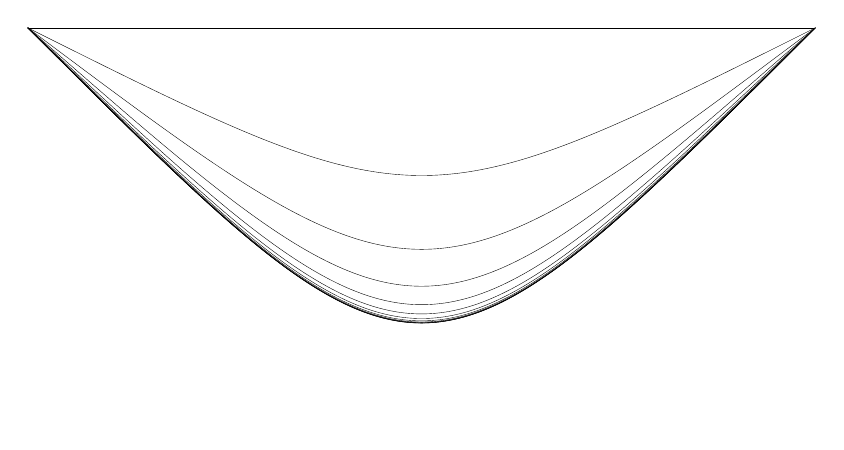
\begin{tikzpicture}[scale=5]
\foreach \i in {0,1,2,...,12}{
	\draw[line width=0.05mm] (-1,1) .. controls (0,1/2^\i) .. (1,1);
}
\end{tikzpicture}
\end{equation*}

A diagram to keep in mind
\begin{equation}
\begin{tikzcd}
\Z^{\infty} \arrow[r, "0"] & \Z^{\infty} \arrow[r, "1"] & \Z^{\infty} \arrow[r, "0"] & \Z^{\infty} \arrow[r, "1"] & \Z^{\infty} \\
\Z^{\infty} \arrow[r, "1"] \arrow[u, "0"] & \Z^{\infty} \arrow[r, "0"] \arrow[u, "0"] & \Z^{\infty} \arrow[r, "1"] \arrow[u, "1"] & \Z^{\infty} \arrow[r, "0"] \arrow[u, "0"] & \Z^{\infty} \arrow[u, "0"]
\end{tikzcd}
\end{equation}

Consider the following general diagram
\begin{equation}
\begin{tikzcd}
A_1 \arrow[r, "s_1"] & A_2 \arrow[r, "s_2"] & B \arrow[r, "t_1"] & C_1 \arrow[r, "t_2"] & C_2 \\
X_1 \arrow[r, "g_1"] \arrow[u, "0"] & X_2 \arrow[r, "g_2"] \arrow[u, "0"] & Y \arrow[r, "h_1"] \arrow[u, "f"] & Z_1 \arrow[r, "h_2"] \arrow[u, "0"] & Z_2 \arrow[u, "0"]
\end{tikzcd}
\end{equation}
